\chapter{Introduktion} \label{sec:intro}
"Droner til monitorering af flerårigt ukrudt i korn"$ $ er et forsknings projekt, oprettet af Miljøstyrelsen, der i samarbejde med Datalogisk institut og institut for Plante- og Miljøvidenskab, har til formål at automatisere detektionen af ukrudt i marker. I dag bekæmpes ukrudt, ved at sprøjte hele marken med pesticider uanset, hvor ukrudtet er placeret. Projektet har til formål at nedsætte forbruget af pesticider, ved hjælp af en drone\footnote{UAV (eng. unmanned aerial vehicle)} udstyret med et kamera. Dronen tager et antal overlappende luftbilleder af en mark. Disse billeder analyseres af en algoritme, der identificere, hvor ukrudtet befinder sig i de enkelte billeder. Resultatet af denne analyse overføres til et globalt koordinatsystem af hele marken, hvilket kan opnås ved at bestemme de geometriske relationer imellem billederne. Det samlede ukrudtskort, vil angive ukrudtets placering og derved, hvor der er behov for pesticider \cite{drone}.
\begin{figure}[H]
    \centering
    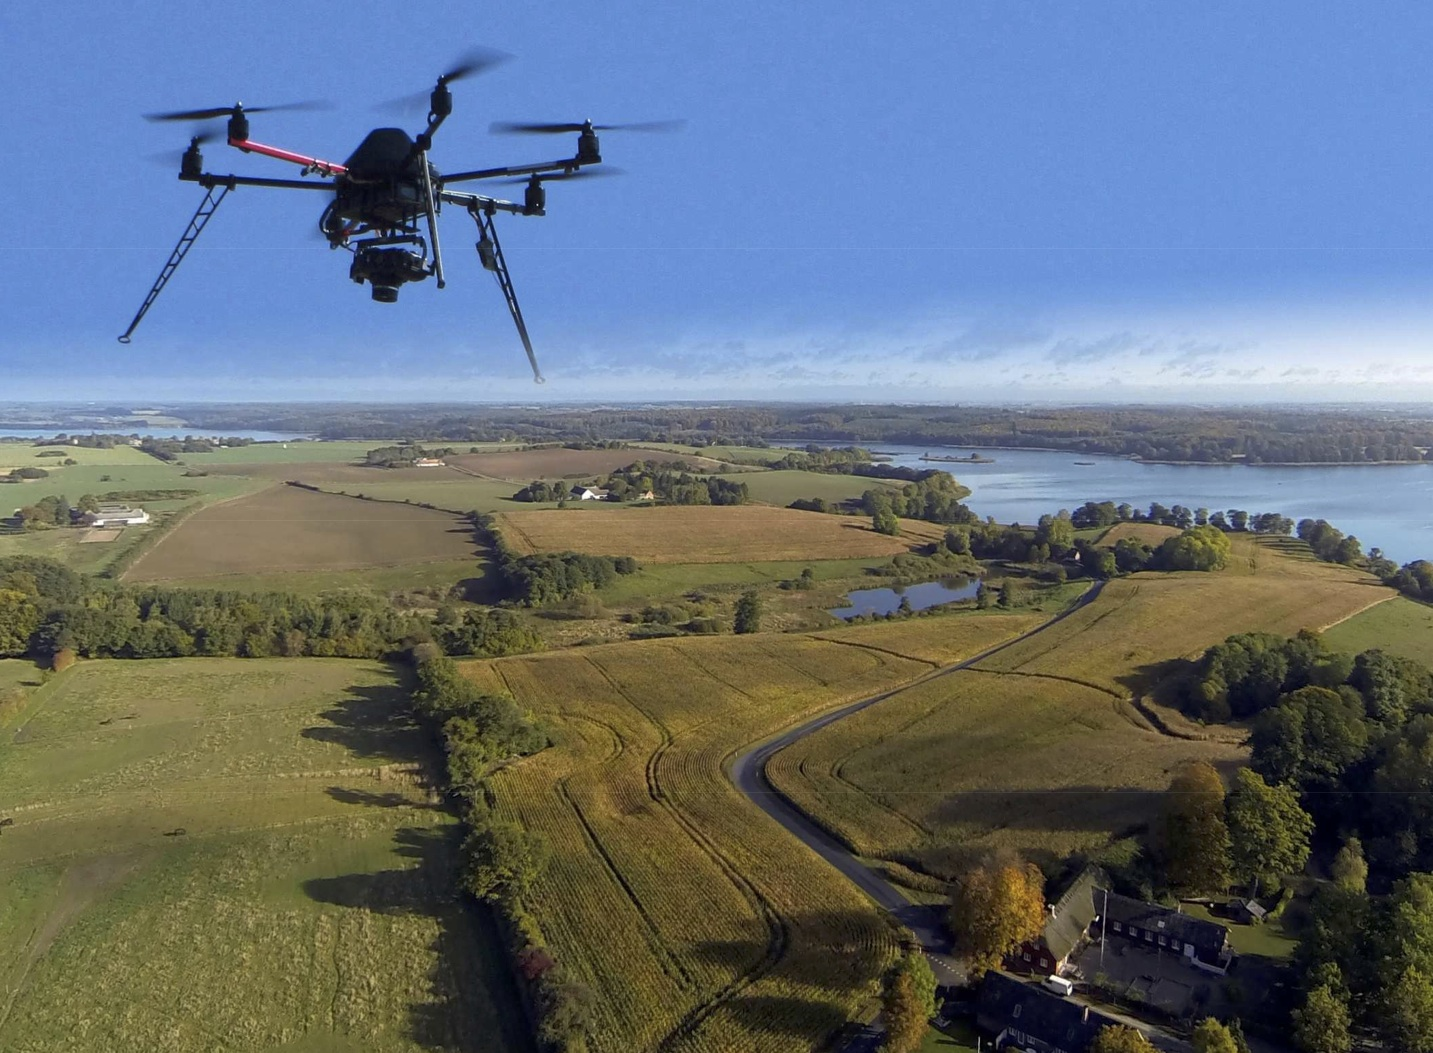
\includegraphics[width=0.45\textwidth]{fig/drone4.jpg}
     \vspace{-0.5em}
    \begin{center}    
    \label{fig:difference}
     \end{center}
     \vspace{-3em}
  \end{figure} \noindent
\section{Opgavens problemfelt} \label{subsec:felt}
Opgavens afsæt i projektet er etablering af korrespondancer, hvilket kan bruges til at estimere de geometriske relationer imellem billederne, igennem homografier. Estimering af de geometriske relationer imellem billederne tillader oprettelsen af ukrudtskortet. Følgende trin beskriver den process der er benyttet til at etablere korrespondancer imellem to billeder, hvilket i denne opgave betegnes som korrespondanceanalyse:
\begin{enumerate}
\item{Interessante punkter udvælges i begge billeder, som resultat af at anvende en række matematiske modeller på billederne. Formålet ved dette stadie er at udvælge  punkter i begge billeder, der repræsentere projektioner af de samme fysiske scenepunkter. Markbillederne overlapper i gennemsnit hinanden med ca. 70 \%, hvilket gør korrespondanceanalysen mulig}
\item{For hvert interessepunkt oprettes en vektor, der beskriver den lokale billedstruktur omkring interessepunktet.}
\item{Beskrivelserne af interessepunkterne i de to billeder, sammenlignes for bestemme, hvilke punkter der korresponderer.}
\end{enumerate}
En nærmere definition af korrespondancebegrebet er givet i sektion \ref{sec:detect}.
\section{Problemformulering} \label{subsec:form}
Med udgangspunkt i litteraturen indenfor
korrespondanceanalyse samt implementering af
flere eksisterende metoder er spørgsmålet, hvilke metoder, der teoretisk og praktisk, bedst anvendes til korrespondanceanalyse af markbilleder.
\subsection{Udvidelse af problemformuleringen}
Der opstilles en beskrivelse af forskellige korrespondanceanalytiske metoder og foretages korrespondanceanalyse af markbillederne, ved implementering af disse metoder. Udvælgelsen af metoder er baseret på hypoteser om, hvad der kræves af metoderne, for at løse korrespondanceproblemet ved markbilleder (afsnit \ref{sec:mark}). Disse hypoteser vil eksperimentelt be - eller afkræftes, og derved give en empirisk forståelse for, hvilke forudsætninger metoderne skal besidde, for at kunne etablere korrespondancer. 
Det undersøges, hvilke metoder der muliggør en løsning af korrespondanceproblemet, samt en komparativ analyse af metodernes præstation.
\subsection{Afgrænsning} \label{subsec:afg}
Projektet sigter på at afprøve allerede eksisterende metoder på markbilleder og ikke at skabe nye metoder. Programmellet konstrueres mht. afklaring af de nævnte problemstillinger
og ikke mhp. efterfølgende at blive anvendt i praksis. De udvalgte metoder implementeres mhp. funktionaliteten. Derfor vil enkelte implementerings detaljer undlades, hvis formålet er at simplificere kompleksiteten.
\section{Implementering}
Alt programmel er skrevet i Python version 2.7. Til det er biblioteket OpenCV anvendt til billedbehandlingsoperationer, som b.la. at læse, vise og gemme billeder. NumPy er anvendt til datarepræsentation, og Matplotlib er brugt til at lave grafer. Relevant programmel er tilføjet i afsnit \ref{sec:app}.
\section{Rapportens Opbygning}
Før projektets anvendte metoder og resultater præsenteres, gives der en kort introduktion af relevante billedbehandlings teknikker, anvendt igennem denne opgave, samt en introduktion til  korrespondanceanalyse. Derefter vil overvejelser, gjort om projektets udfordringer, præsenteres. Til sidst vil anvendte metoder gennemgås, efterfulgt af en præsentation og diskussion af opgavens resultater.